\section{Analysis Results}

\subsection{Belt Drive}\label{bd_fea}

% include software pics

\subsection{Wheel Shaft}\label{ws_fea}

% fea

\subsection{Pivot}\label{pivot_fea}

% fea

\subsection{Drive Box}\label{box_fea}

\begin{figure}[htbp]
\centering
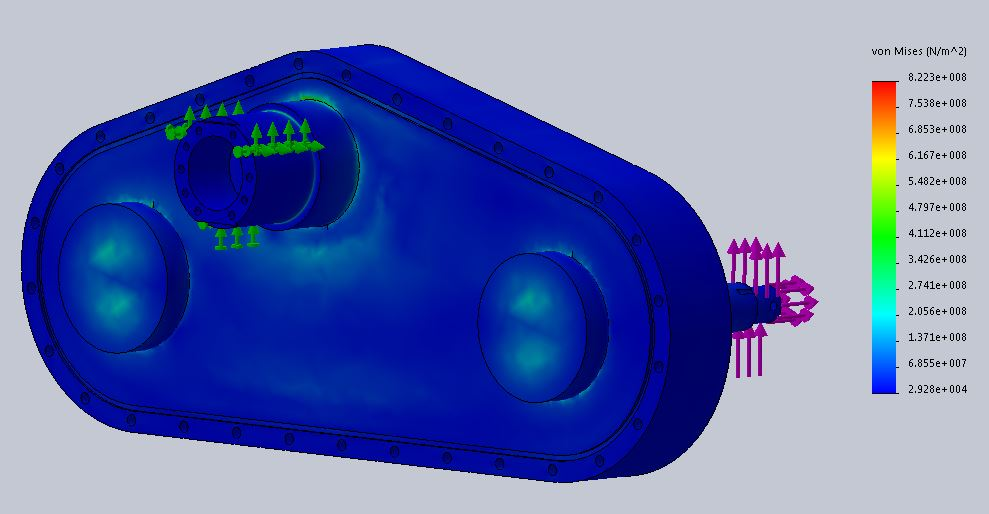
\includegraphics[width=\textwidth]{images/drive_box_stress_fea}
\caption[Drive Box FEA Stress Results]{FEA stress results for drive box analysis. Maximum stress is 82.23 MPa.}
\label{fig:box_fea1}
\end{figure}

\begin{figure}[htbp]
\centering
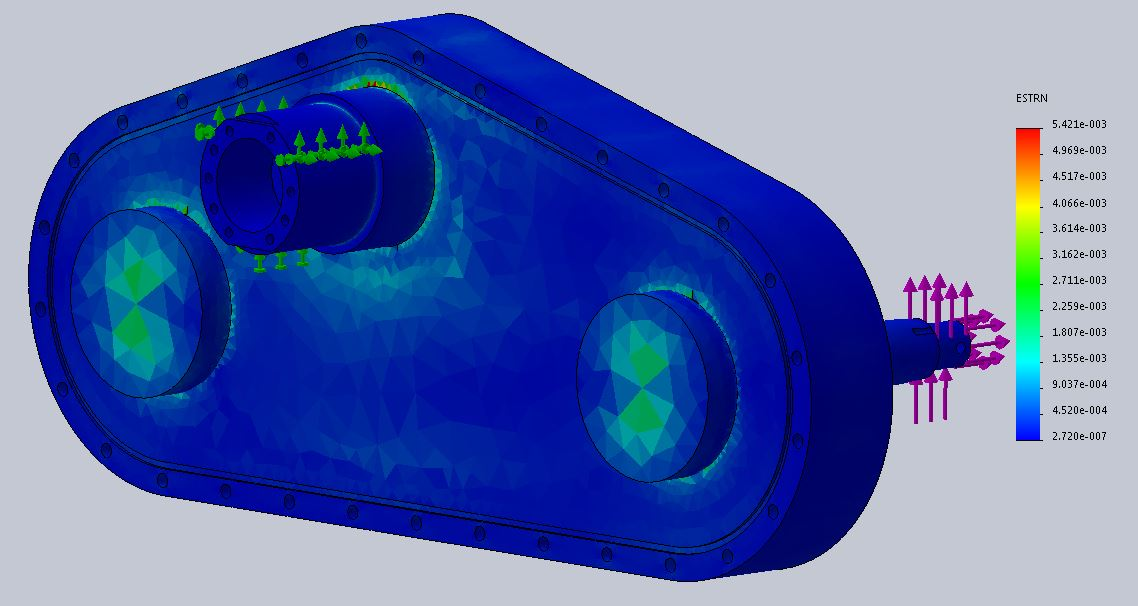
\includegraphics[width=\textwidth]{images/drive_box_strain_fea}
\caption[Drive Box FEA Strain Results]{FEA strain results for drive box analysis. Maximum strain is 5 mm.}
\label{fig:box_fea2}
\end{figure}

\subsection{Idler}

\begin{figure}[htbp]
\centering
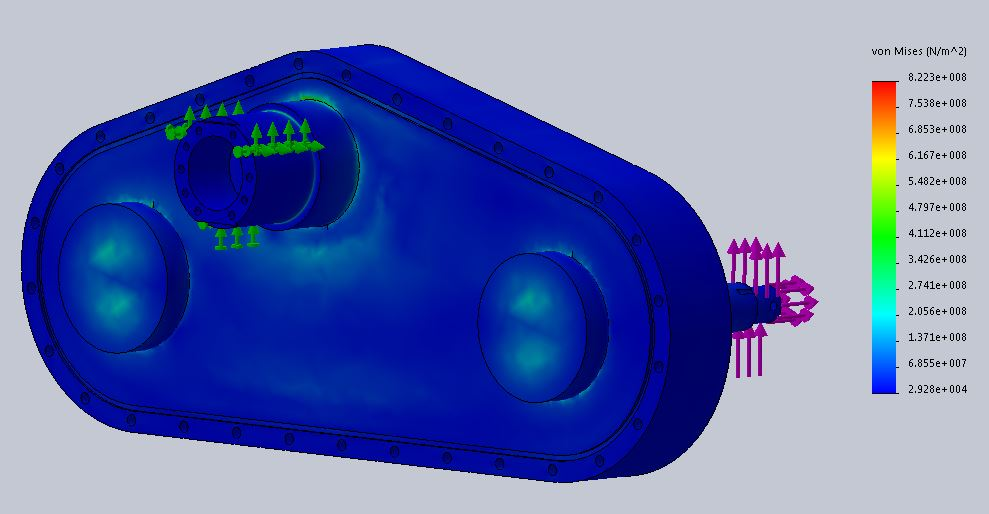
\includegraphics[width=\textwidth]{images/drive_box_stress_fea}
\caption[Idler FEA Stress Results]{FEA stress results for drive box analysis. Maximum stress is 82.23 MPa.}
\label{fig:idler_fea1}
\end{figure}

\begin{figure}[htbp]
\centering
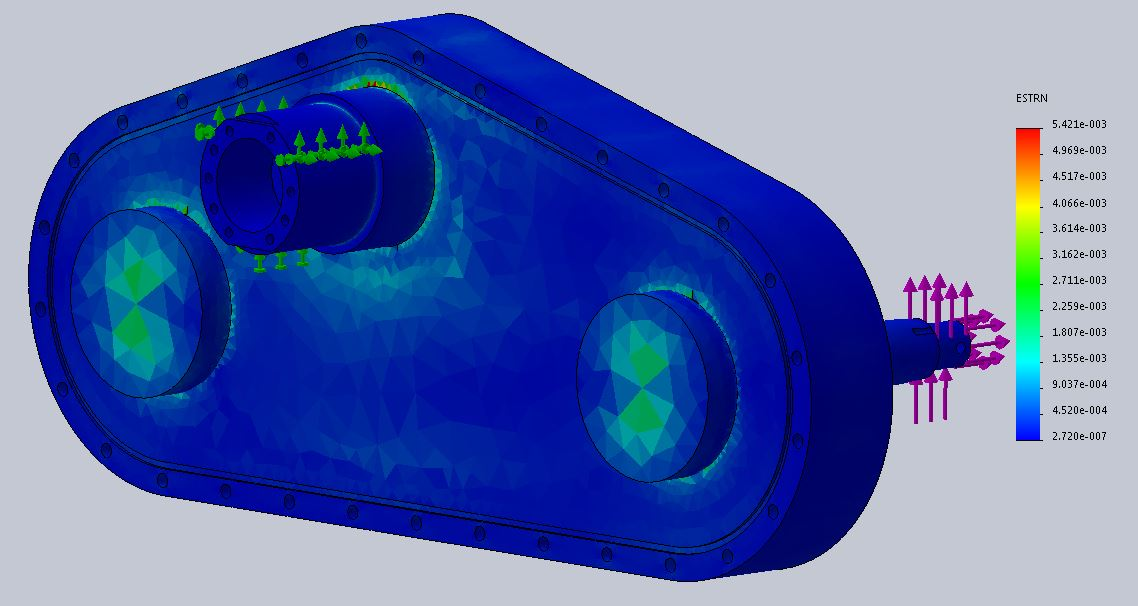
\includegraphics[width=\textwidth]{images/drive_box_strain_fea}
\caption[Idler FEA Strain Results]{FEA strain results for drive box analysis. Maximum strain is 5 mm.}
\label{fig:idler_fea2}
\end{figure}

\subsection{Battery Rack}\label{br_fea}